\section[Electrical conductivity and the Hall effect]{\hyperlink{toc}{Electrical conductivity and the Hall effect}}


\subsection{Electrical conductivity in the Drude model}

\begin{itemize}
    \item Next, let's consider when we have a non-zero electrical field (with $\mathbf{B}$ still 0):
    
    \[ \vec{E} \neq 0, \quad \vec{B} = 0 \]

    Equation of motion:

    \[ \dv{\vec{p}}{t} = -e \vec{E} - \frac{\vec{p}(t)}{\tau} \]

    \item We can now define the conductivity of a metal, $\sigma$, which is the constant of proportionality between the current density $\vec{j}$, and the applied electric field $\vec{E}$.
    
    \begin{center}
        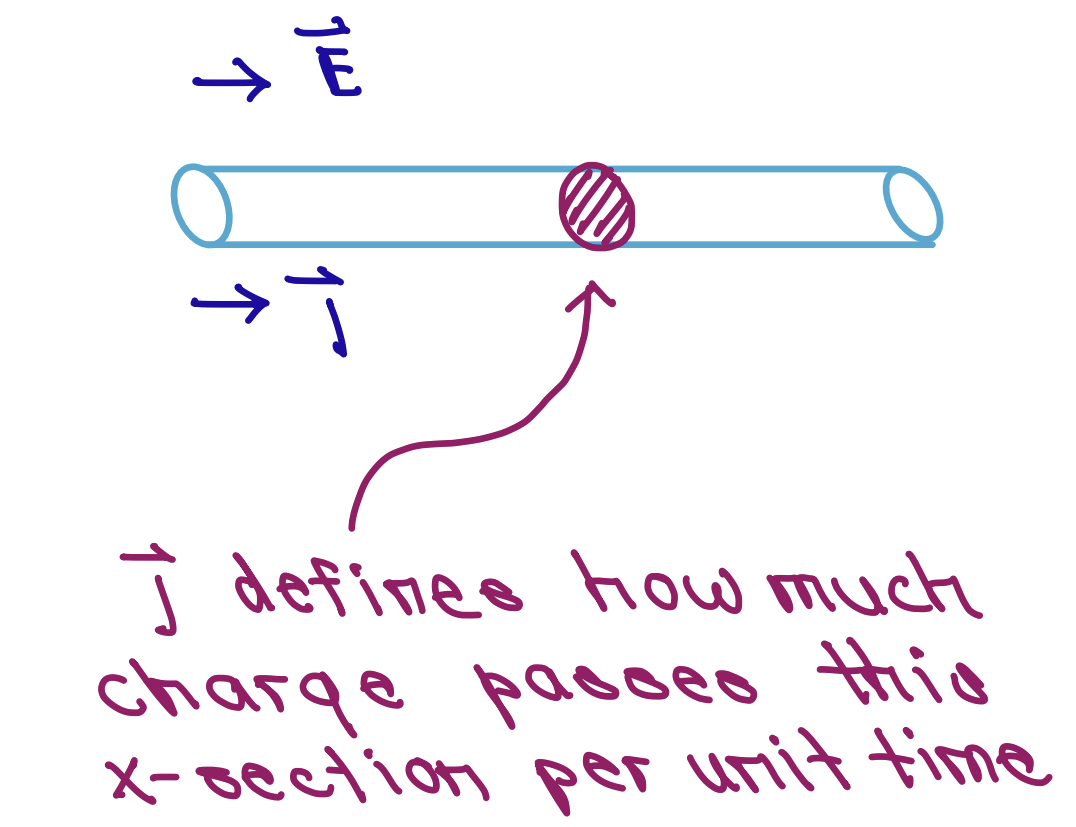
\includegraphics[width = 0.3 \linewidth]{Images/current-density.png}
    \end{center}

    where

    \[\vec{j} = \text{current density} \]
    
    which is the charge per unit time per unit area

    \[ \vec{j} = - n e \vec{v} \]

    where $n$ is the density of electrons   

    \[ \brackets*{e^-/m^3}\brackets*{C/e^-} \brackets*{m/s} = \frac{C}{m^2 \cdot s} \]

    \[ \vec{j} = \frac{e^2 n \tau}{m} \vec{E} \Rightarrow \boxed{\sigma = \frac{e^2 n \tau}{m}} \text{ units } \brackets*{\Omega^{-1} m^{-1}}\]

    \item Thus we can define resistivity $\rho$ as the inverse of conductivity:
    
    \[ \boxed{\rho = \frac{1}{\sigma} }  \text{ units } \brackets*{\Omega m}\]

    \item If the resistivity of a metal is given by $\rho = \frac{1}{\sigma} = \frac{m}{e^2 n \tau}$, then decreasing the collision rate ($\frac{1}{\tau}$), will increase $\tau$ and thus lower the resistance.
    
    \item Note that increasing or decreasing the size of the sample does not change the resistivity. $\rho$ is \emph{intrinsic} (depends on material properties), while $R= \rho \cdot \frac{L}{A}$ is \emph{extrinsic} (depends on the size and shape of the sample).

    \item \[ \sigma \propto \tau \Rightarrow \uparrow \tau \text{ means fewer collisions per electron (lower collision rate)} \]
\end{itemize}

\subsection{Hall Effect}
\begin{center}
    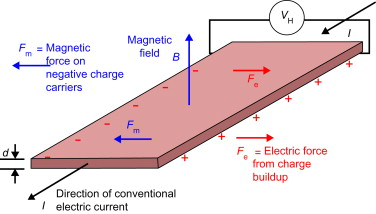
\includegraphics[width = 0.4 \linewidth]{Images/hall-effect.jpg}
\end{center}

\begin{itemize}

    \item Next, we can apply an electric and magnetic field to our metal simultaneously (in perpendicular directions). By convention, we will always apply $\mathbf{B}$ in the $z$ direction. 
    
    \item Recall -- equation of motion:
    
    \[ \dv{\vec{p}}{t} = -e \left( \vec{E} + \vec{v} \times \vec{B} \right) + \frac{\vec{p}(t)}{\tau} \]

    \item If we again assumee steady state, we get:
    \[ \vec{E} = \left( \frac{m}{ne^2 \tau} \right) \vec{j} + \left( \frac{1}{ne} \right) \vec{j} \times \vec{B} \]

    where the first term is "longitudinal"  and the second term is off diagonal.

    \item We can define a 3 x 3 resistivity matrix and we find that the application of a $\mathbf{B}$ field deflects the electrons causing a measurable potential difference in the orthogonal direction -- this is the Hall effect.
    
    \[ \vec{B} \parallel \hat{z}, \quad \vec{j} \text{ can be applied along } \hat{x}, \hat{y}, or \hat{z} \]
        
    \[ \rho_{xx} = \rho_{yy} = \rho_{zz} = \frac{m}{ne^2 \tau} \]

    Hall resistivity:

    \[ \boxed{ \rho_{xy} = -\rho_{yx} = \frac{B}{ne}} \]

    \item Note that in steady state the current flows in only one spatial direction.
    
    \begin{itemize}
        \item In the steady state, once the potential difference is established in the transverse direction, no additional current flows in that direction.
        \[ \text{i.e.} \quad |\vec{F}_{\text{e}}| = |\vec{F}_{\text{B}}| \quad \text{ on the previous diagram} \]

        
        \item current only flows in the "applied" direction.
    \end{itemize}

    \item KEY! Whereas the longitudinal resistivity ($\rho_{xx}$) depends on both $\tau$ and $n$ -- so that they cannot be uniquely determined -- \textbf{the Hall resistivity depends only on n}, so we can determine the number of conduction electrons. 
    \item We can define the Hall coefficient, $R_H$:
    \[ R_H = \frac{-1}{ne} = \frac{-\rho_{xy}}{|B|} \quad \text{ units } \brackets*{m^3/C}\]

    note: "normal" meteals have a negative $R_H$ (NOT a resistance).

    \begin{center}
        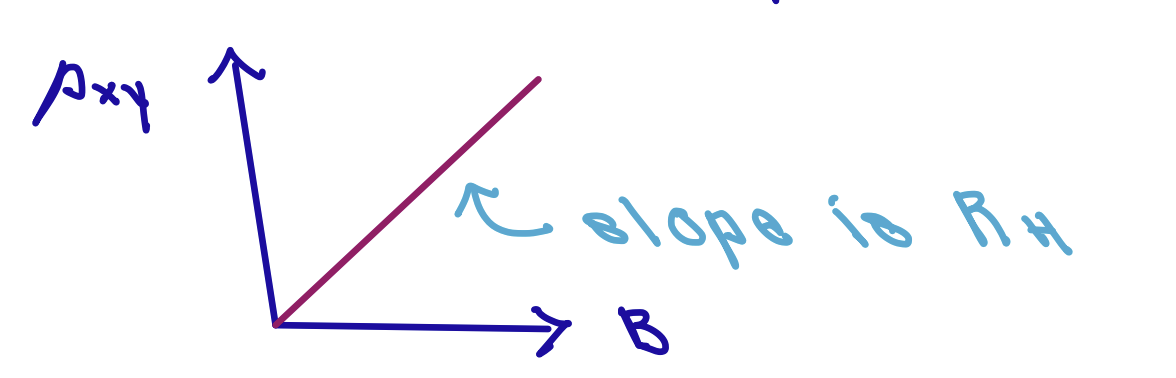
\includegraphics[width = 0.4 \linewidth]{Images/hall-effect-slope.png}
    \end{center}

    \item Some metals have a positive Hall coefficient -- seeming to imply the existence of a positively charged carrier of electrical current. This is forshadowing for later in the course when we will get introduced to the concept of holes in semiconductors.

    \item The Hall coefficient $R_H$ for copper (good metal) is of order 0.1 $mm^3/C$ and its resistivity at RT is of order $10^{-8} \Omega m$. The order of magnitude of the scattering time, $\tau$.
    
    \[ R_H = 0.1 mm^3/C = 10^{-10} m^3/C = \frac{-1}{n e} \]

    \[ \rho = \frac{1}{\sigma} = 10^{-8} \Omega m = \frac{m}{n e^2 \tau} \]

    \[ \tau = \frac{-m R_H}{e^2 \rho} = \frac{-\paren*{10^{-30}\, \text{kg}} \paren*{10^{-10} m^{3}/C}}{\paren*{-10^{-19} C} \paren*{10^{-8} \Omega m}} = 10^{-13} s \]

    \item Average metal $\approx$ 10$^{-14}$ s, so this is reasonable. Scattering time is extraordinarile short. 
\end{itemize}